\section{Pulsar Evolution}
\seclabel{pulsar_evolution}

\begin{figure}[htbp]
  \centering
    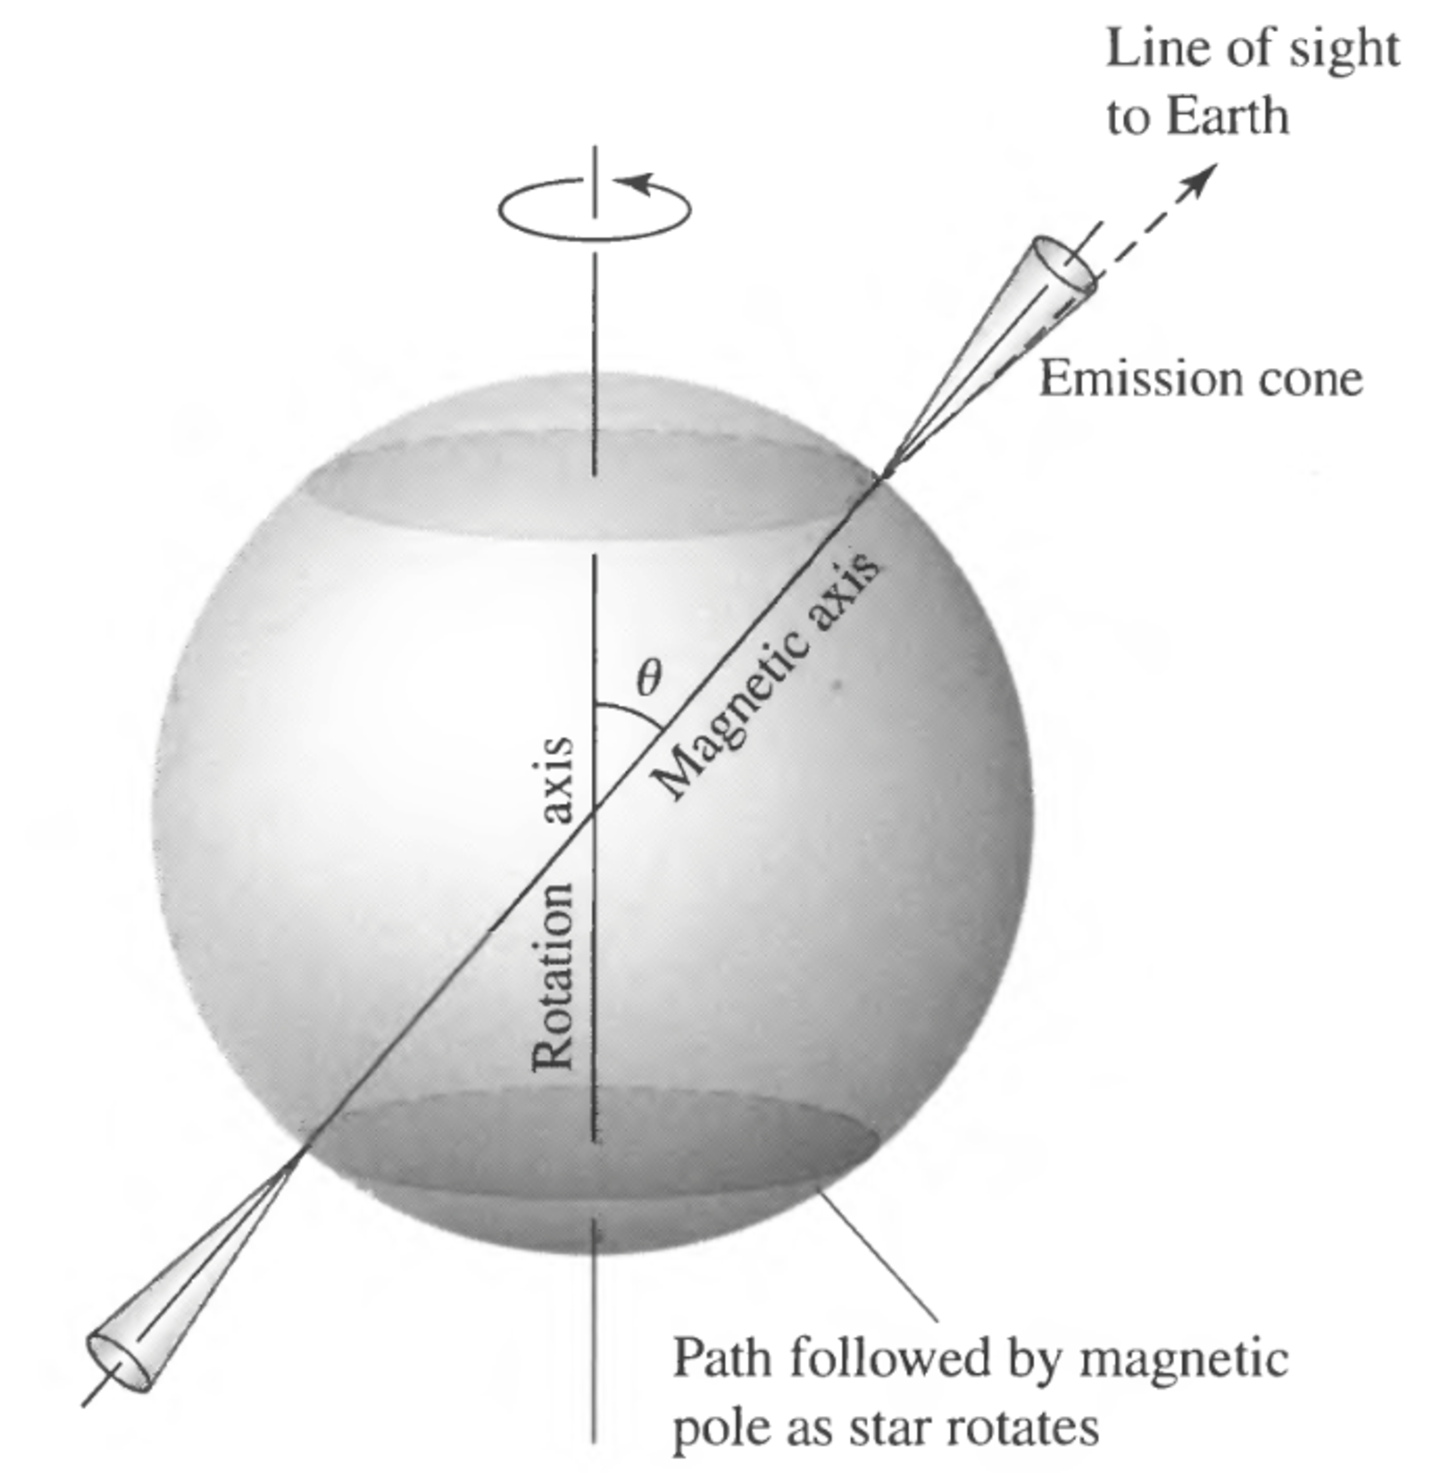
\includegraphics[width=0.5\textwidth]{chapters/pulsar_pwn_system/figures/pulsar_model.pdf}
    \caption{The rotating dipole model of a pulsar. This figure is taken
    from \citep{carroll_2006_introduction-modern}.}
  \figlabel{pulsar_model}
\end{figure}

The simplest model of a pulsar is that it is a rotating dipole magnet
with the rotation axis and the magnetic axis offset by an angle
$\PulsarRotationAngle$ (see \figref{pulsar_model}).  The energy output
from the pulsar is assumed to come from rotational kinetic energy
stored in the neutron star which is released as the pulsar spins down.

For a pulsar, both the period \period and the period derivative
$\perioddot=d\period/d\time$ can be directly observed.  Except in a
few \acp{MSP} which are being sped up through accretion \cite[see for
example][]{falanga_2005_integral-observations}), pulsars are slowing down
($\perioddot<0$).  We write the rotational kinetic energy as
\begin{equation}\eqnlabel{rotational_energy}
  \energyrotational = \tfrac{1}{2} I \PulsarAngularFrequency^2
\end{equation}
where $\PulsarAngularFrequency = 2\pi/\period$ is the angular frequency
of the pulsar and \momentofinertia is the moment of inertia.
For a uniform sphere,
\begin{equation}
  \momentofinertia = \frac{2}{5} M R^2.
\end{equation}
Assuming a canonical pulsar (see \seclabel{neutron_star_formation}),
we find a canonical moment of inertia of
$\momentofinertia=10^{45}\unitspace\gram\unitspace\cm^{-2}$.

We make the connection between the pulsar's spin-down
energy and the rotational kinetic energy as $\energydot
= - \derivative\energyrotational/\dtime$.
\eqnref{rotational_energy} can be rewritten as
\begin{equation}\eqnlabel{edot_from_rotation}
  \energydot = I \PulsarAngularFrequency \PulsarAngularFrequencyDot.
\end{equation}
It is believed that as the pulsar spins down, the this rotational energy
is released as pulsed electromagnetic radiation and also as a wind of
electrons and positrons accelerated in the magnetic field of the pulsar.

If the pulsar were a pure dipole magnet, its radiation would be described
as \citep{gunn_1969_magnetic-dipole}
\begin{equation}\eqnlabel{edot_pure_dipole}
  \energydot = \frac{2\MagneticField^2 \PulsarRadius^6 
  \PulsarAngularFrequency^4 \sin^2\PulsarRotationAngle}{
  3\speedoflight^3}.
\end{equation}
Combining equations \eqnref{edot_from_rotation} and
\eqnref{edot_pure_dipole}, we find that for a pure dipole magnet,
\begin{equation}\eqnlabel{breaking_index_dipole}
  \PulsarAngularFrequencyDot \propto \PulsarAngularFrequency^3.
\end{equation}

In the few situations where this relationship has been
conclusively measured, this relationship does not hold
\citep[See][ and references therein]{espinoza_2011_braking-index}.
We generalize \eqnref{breaking_index_dipole} as:
\begin{equation}\eqnlabel{angular_frequency_derivative_relation}
  \PulsarAngularFrequencyDot \propto \PulsarAngularFrequency^\breakingindex
\end{equation}
where $\breakingindex$ is what we call the breaking index.
We solve \eqnref{angular_frequency_derivative_relation}
for \breakingindex by taking the derivative:
\begin{equation}
  \breakingindex = \frac{\PulsarAngularFrequency \PulsarAngularFrequencyDotDot}{\PulsarAngularFrequencyDot^2}
\end{equation}

The breaking index is hard to measure due to timing noise and glitches
in the pulsar's phase. To this date, it has been measured in eight
pulsars \cite{espinoza_2011_braking-index}, and in all situations
$\breakingindex<3$. This suggests that there are additional processes
besides magnetic dipole radiation that contribute to the energy release
\citep{blandford_1988_interpretation-pulsar}.

\eqnref{angular_frequency_derivative_relation} is a Bernoulli differential
equation which can be integrated to solve for time:
\begin{equation}\eqnlabel{pulsar_age}
  T = \frac{\period}{(\breakingindex-1) \absval{\perioddot}}
  \left(
  1-\left(\frac{\period_0}{\period}\right)^{(\breakingindex-1)}
  \right)
\end{equation}
For a canonical $\breakingindex=3$ pulsars which is relatively old
$\period_0 \ll \period$, we obtain what is called the characteristic
age of the pulsar:
\begin{equation}
  \PulsarAge = \period/2\perioddot.
\end{equation}

Using \eqnref{edot_from_rotation} and \eqnref{breaking_index_dipole},
we can solve for the spin-down evolution of the pulsar as a function of
time \citep{pacini_1973_evolution-supernova}:
\begin{equation}\eqnlabel{energy_dot_vs_time}
    \energydot(t) = \energydot_0
    \left(
    1 + \frac{\time}{\SpinDownTimescale}
    \right)^{-\frac{(\breakingindex+1)}{(\breakingindex-1)}}.
\end{equation}
Here,
\begin{equation}
  \SpinDownTimescale \equiv \frac{\period_0}{(\breakingindex-1)\absval{\perioddot_0}}.
\end{equation}

\eqnref{edot_from_rotation}, \eqnref{pulsar_age}, and
\eqnref{energy_dot_vs_time} show us that given the current period,
period derivative, and breaking index, we can calculate the pulsar's
age and energy-emission history.

In a few situations, the pulsar's age is well known and the
breaking index can be measured, so $\period_0$ can be inferred. See
\cite{kaspi_2002_constraining-birth} for a review of the topic. For
other sources, attempts have been made to infer the initial spin-down
age based on the dynamics of an associated \acs{SNR}/\ac{PWN}
\citep{van-der-swaluw_2001_inferring-initial}.

Finally, if we assume dipole radiation is the only source of energy
release, we can combine equation \eqnref{edot_from_rotation} and
\eqnref{edot_pure_dipole} to solve for the magnetic field:
\begin{equation}
  \MagneticField = \sqrt{\frac{3\momentofinertia\speedoflight^3}{
  8\pi^2\PulsarRadius^6\sin^2\PulsarRotationAngle}\period\perioddot}
  = 3.2\times 10^{19} \sqrt{\period\perioddot} \unitspace\gauss
\end{equation}
where in the last step we assumed the canonical values of
$\momentofinertia=10^{45}\unitspace\gram\unitspace\cm^{-2}$,
$\PulsarRadius=10\unitspace\km$, $\PulsarRotationAngle=90\degree$, and we
assume that $\period$ is measured in units of seconds.  For example,
for the Crab nebula, $\period\approx33\unitspace\millisecond$
\citep{staelin_1968_pulsating-radio} and
$\perioddot\approx36\unitspace\nanosecond$
per day \citep{richards_1969a_period-pulsar} so
$\MagneticField\approx10^{12}\unitspace\gauss$.
